% !TEX program = xelatex
\documentclass[10pt,letterpaper,twocolumn]{article}

% === GEOMETRY ===
\usepackage[top=0.75in, bottom=0.75in, left=0.75in, right=0.75in]{geometry}

% === FONTS ===
\usepackage{fontspec}
\usepackage{unicode-math}
\usepackage{xeCJK}
\setCJKmainfont{Droid Sans Japanese}

\setmainfont{Latin Modern Roman}
\setsansfont{Latin Modern Sans}

% Custom AC fonts
\newfontfamily\acbold{ywft-processing-bold}[
  Path=../../system/public/type/webfonts/,
  Extension=.ttf
]
\newfontfamily\aclight{ywft-processing-light}[
  Path=../../system/public/type/webfonts/,
  Extension=.ttf
]
\newfontfamily\kidlispfont{ComicRelief-Regular}[
  Path=../arxiv-kidlisp/fonts/,
  Extension=.ttf
]
\newfontfamily\kidlispbold{ComicRelief-Bold}[
  Path=../arxiv-kidlisp/fonts/,
  Extension=.ttf
]
\setmonofont{Latin Modern Mono}[Scale=0.85]

% === PACKAGES ===
\usepackage{xcolor}
\usepackage{titlesec}
\usepackage{enumitem}
\usepackage{booktabs}
\usepackage{tabularx}
\usepackage{fancyhdr}
\usepackage{hyperref}
\usepackage{graphicx}
\graphicspath{{figures/}{../arxiv-kidlisp/figures/}}
\usepackage{ragged2e}
\usepackage{microtype}
\usepackage{listings}
\usepackage{natbib}
\usepackage[colorspec=0.92]{draftwatermark}

% === COLORS (AC palette) ===
\definecolor{acpink}{RGB}{180,72,135}
\definecolor{acpurple}{RGB}{120,80,180}
\definecolor{acdark}{RGB}{64,56,74}
\definecolor{acgray}{RGB}{119,119,119}
\definecolor{klbrand}{RGB}{205,92,155}
\definecolor{klcyan}{RGB}{112,214,255}
\definecolor{kldark}{RGB}{48,43,58}
\definecolor{draftcolor}{RGB}{205,92,155}

% === DRAFT WATERMARK ===
\DraftwatermarkOptions{
  text=作業草稿,
  fontsize=3cm,
  color=draftcolor!18,
  angle=45,
  pos={0.5\paperwidth, 0.5\paperheight}
}

% === KIDLISP SYNTAX COLORS ===
\definecolor{klfn}{RGB}{0,136,170}
\definecolor{klform}{RGB}{119,51,170}
\definecolor{klrepeat}{RGB}{170,0,170}
\definecolor{klnum}{RGB}{204,0,102}
\definecolor{klstr}{RGB}{170,120,0}
\definecolor{klcmt}{RGB}{102,102,102}
\definecolor{klmath}{RGB}{0,136,0}
\definecolor{klvar}{RGB}{204,102,0}
\definecolor{klembed}{RGB}{0,136,0}

% KidLisp inline color macros
\newcommand{\kn}[1]{\textcolor{klnum}{#1}}
\newcommand{\kt}[1]{\textcolor{klstr}{#1}}
\newcommand{\kv}[1]{\textcolor{klvar}{#1}}
\newcommand{\ke}[1]{\textcolor{klembed}{\textbf{#1}}}
\newcommand{\km}[1]{\textcolor{klmath}{#1}}

% === HYPERREF ===
\hypersetup{
  colorlinks=true,
  linkcolor=acpurple,
  urlcolor=acpurple,
  citecolor=acpurple,
  pdfauthor={@jeffrey},
  pdftitle={KidLisp カード：1枚のカードに収まるプログラム},
}

% === SECTION FORMATTING ===
\titleformat{\section}
  {\normalfont\bfseries\normalsize\uppercase}
  {\thesection.}
  {0.5em}
  {}
\titlespacing{\section}{0pt}{1.2em}{0.3em}

\titleformat{\subsection}
  {\normalfont\bfseries\small}
  {\thesubsection}
  {0.5em}
  {}
\titlespacing{\subsection}{0pt}{0.8em}{0.2em}

% === HEADER/FOOTER ===
\pagestyle{fancy}
\fancyhf{}
\renewcommand{\headrulewidth}{0pt}
\fancyhead[C]{\footnotesize\color{acpink}\textit{作業草稿 --- 引用不可}}
\fancyfoot[C]{\footnotesize\thepage}

% === CUSTOM COMMANDS ===
\newcommand{\acdot}{{\color{acpink}.}}
\newcommand{\kidlisp}{\textsc{KidLisp}}

% === LISTINGS ===
\lstdefinelanguage{kidlisp}{
  morekeywords=[1]{wipe,ink,line,box,circle,tri,plot,flood,shape,zoom,scroll,spin,blur,contrast,embed,layer,width,height,frame,time,wiggle,melody,mic,suck,sort,form,trans,cube,move,scale,hop,overtone,resolution,write,text,type,stamp,paste,point,poly,noise,fade,pan,unpan,mask,unmask,flip,crawl,left,right,up,down,goto,face,outline,fill,stroke},
  morekeywords=[2]{def,let,if,cond,once,later,lambda,do},
  morekeywords=[3]{repeat},
  morekeywords=[4]{random,sin,cos,tan,floor,ceil,round,abs,sqrt,min,max},
  sensitive=true,
  morecomment=[l]{;},
  morestring=[b]",
  escapeinside={|}{|},
}
\lstset{
  language=kidlisp,
  basicstyle=\ttfamily\small,
  keywordstyle=[1]\color{klfn}\bfseries,
  keywordstyle=[2]\color{klform}\bfseries,
  keywordstyle=[3]\color{klrepeat}\bfseries,
  keywordstyle=[4]\color{klmath},
  commentstyle=\color{klcmt}\itshape,
  stringstyle=\color{klstr},
  breaklines=true,
  frame=single,
  rulecolor=\color{acgray!30},
  backgroundcolor=\color{acgray!5},
  xleftmargin=0.5em,
  xrightmargin=0.5em,
  aboveskip=0.5em,
  belowskip=0.5em,
}

\lstdefinelanguage{python}{
  morekeywords={def,return,import,from,class,if,else,for,in,with,as,try,except,None,True,False,self,and,or,not,lambda,yield,pass,break,continue,raise,while},
  sensitive=true,
  morecomment=[l]{\#},
  morestring=[b]",
  morestring=[b]',
}
\lstset{
  language=kidlisp,
}

% === LIST SETTINGS ===
\setlist[itemize]{nosep, leftmargin=1.2em, itemsep=0.1em}
\setlist[enumerate]{nosep, leftmargin=1.2em}

% === COLUMN SEPARATION ===
\setlength{\columnsep}{1.8em}

% === PARAGRAPH SETTINGS ===
\setlength{\parindent}{1em}
\setlength{\parskip}{0.3em}

\tolerance=800
\emergencystretch=1em
\hyphenpenalty=50

\begin{document}

% ============ TITLE BLOCK ============

\twocolumn[{%
\begin{center}

\includegraphics[height=4em]{pals}\par\vspace{0.5em}
{\kidlispbold\fontsize{24pt}{28pt}\selectfont\color{kldark} Kid{\color{klbrand}Lisp} カード}\par
\vspace{0.2em}
{\kidlispfont\fontsize{11pt}{13pt}\selectfont\color{klbrand} 1枚のカードに収まるプログラム}\par
\vspace{0.6em}
{\normalsize @jeffrey}\par
{\small\color{acgray} Aesthetic\acdot Computer}\par
{\small\color{acgray} ORCID: \href{https://orcid.org/0009-0007-4460-4913}{0009-0007-4460-4913}}\par
\vspace{0.3em}
{\small\color{acpurple} \url{https://kidlisp.com} \enspace$\cdot$\enspace \url{https://aesthetic.computer}}\par
\vspace{0.6em}
\rule{\textwidth}{1.5pt}
\vspace{0.5em}
\end{center}

\begin{center}
{\small\color{acpink}\textbf{[ 作業草稿 --- 引用不可 ]}}
\end{center}
\vspace{0.3em}

\begin{quote}
\small\noindent\textbf{要旨。}
\kidlisp{} のプログラムは短い。典型的なプログラムはわずか2--4行のS式で完全なビジュアル構図を生み出す——スターバースト、螺旋、パッチワーク、フラクタル。この短さは偶然ではなく意図的な設計である。言語がユーザー定義関数、再帰、抽象化メカニズムを省略しているため、プログラムはフラットで可読なままである。このフラットさがプログラムと物理カードの間に自然な対応を生み出すことに気づいた。\kidlisp{} プログラムとそのソースコード、レンダリング出力は1枚の印刷カード上に共存できる。本稿では\emph{KidLisp Cards}フォーマット——ビジュアルカテゴリ別に整理されたプログラムカードのデッキ——と、ブラウザ外でカード画像を生成するPythonレンダリングパイプライン（PILベースのインタプリタ）を記述する。カードが現在何であるか（キュレーションされたビジュアル公案のノートブック）、将来何になりうるか（トレーディングカード、教育シーケンス、印刷スコア、メールアート）、そしてカードの制約が言語設計にどうフィードバックするかを論じる。
\end{quote}
\vspace{0.5em}
}]

% ============ 1. はじめに ============

\section{はじめに}

ほとんどのプログラミング言語は、インデックスカード1枚に印刷するには長すぎるプログラムを生み出す。これは抽象化の帰結である。汎用プログラミング言語はプログラムを関数、クラス、モジュール、ファイルに分解することを促す。プログラムはコードベース全体に散らばる。全体像を捉える単一のアーティファクトは存在しない。

\kidlisp{} は異なる。プログラムは通常1--6行である。完全なアニメーションシーン、幾何学パターン、再帰フラクタル、モアレ干渉パターンがわずか数個のS式で済む。これは制限ではなく設計上の選択である。\kidlisp{} はユーザー定義関数、再帰（\texttt{later} を介する場合を除く）、可変データ構造、インポートを省略している。プログラムは描画コマンド、ループ、条件のフラットなシーケンスである。

このフラットさが機会を生む。プログラムのソースコードが1枚のカードに収まり、そのプログラムのビジュアル出力も同じカードに収まるなら、カードは自己完結したアーティファクトとなる——手に取り、人に渡し、壁に貼り、郵送できるプログラム。カードは文書であると同時に実行可能である。それは\emph{スコア}——ビジュアルイベントを生成する指示書である。

本稿ではKidLisp Cardsフォーマット（\S\ref{sec:format}）、オフラインレンダリングパイプライン（\S\ref{sec:pipeline}）、現在のカードカタログ（\S\ref{sec:catalog}）、レイアウトバリエーションとその社会的・物理的アフォーダンス（\S\ref{sec:layouts}）、フォーマットの投機的未来（\S\ref{sec:futures}）を記述する。

% ============ 2. カードフォーマット ============

\section{カードフォーマット}
\label{sec:format}

KidLispカードには3つの要素がある：

\begin{enumerate}
  \item \textbf{タイトル。}ビジュアル出力のイメージを喚起する短い名前：``Starburst''、``Honeycomb''、``Spiral Walk''。
  \item \textbf{レンダリング出力。}ピクセルアート画像（デフォルト解像度160$\times$120、シャープなエッジを維持するためニアレストネイバー補間で3$\times$拡大）。
  \item \textbf{ソースコード。}完全な \kidlisp{} プログラム、通常1--4行、画像の下に等幅フォントで表示。
\end{enumerate}

カードは自己完結している。ソースコードを読める人なら誰でも、任意の \kidlisp{} インタプリタで画像を正確に再現できる。外部依存なし、インポートなし、設定なし。プログラム\emph{が}カードである。

\subsection{カードサイズ}

レンダリング画像は160$\times$120ピクセルのキャンバス（4:3比率）を占め、\kidlisp{} のデフォルト解像度と一致する。3$\times$拡大で480$\times$360ピクセルの画像となり、画面表示に適する。印刷用にはカードサイズは4$\times$6インチ（標準インデックスカード/ポストカード）で、画像が上部、ソースコードが下部。

\subsection{良いカードとは}

すべての \kidlisp{} プログラムが良いカードになるわけではない。最良のカードは以下の特徴を共有する：

\begin{itemize}
  \item \textbf{短い。}1--4行。ソースコードが画像の下に快適に収まらなければ、そのプログラムはフォーマットに対して長すぎる。
  \item \textbf{驚き。}出力はソースコードが示唆する以上に複雑または美しくあるべき。モアレパターンを生成する3行のプログラムは注目に値する。
  \item \textbf{可読性。}読者はプログラムを実行せずにソースコードから出力をたどれるべき。コードと画像の結びつきは識別可能であるべき——たとえ即座に明白でなくとも。
  \item \textbf{独立性。}\texttt{\$code} 埋め込みなし、外部状態なし。カードは単独で動作しなければならない。
\end{itemize}

\begin{figure}[t]
\centering
\fbox{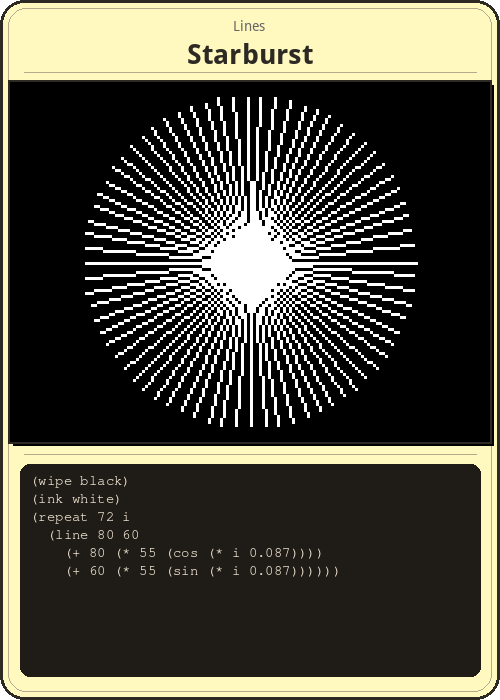
\includegraphics[width=0.47\columnwidth]{card-starburst.png}}%
\hfill%
\fbox{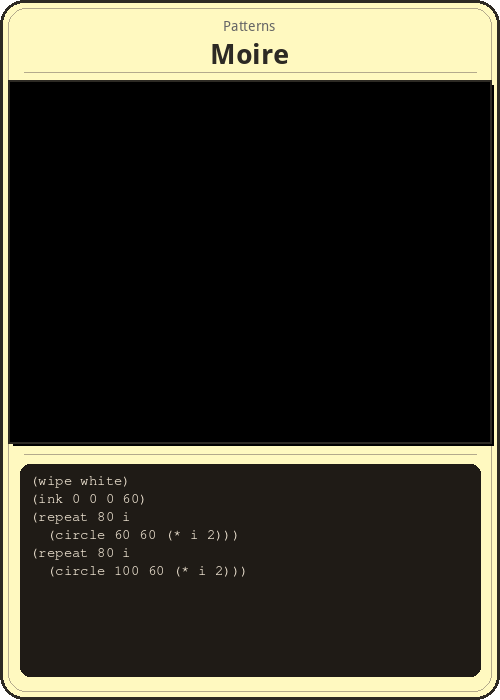
\includegraphics[width=0.47\columnwidth]{card-moire.png}}
\caption{Pythonインタプリタでレンダリングされた2枚のプログラムカード：``Starburst''（72本の放射状線、3行のコード）と``Moir\'{e}''（重なる同心円、3行）。これらは単純な例であり——カードフォーマットの構造を示すが、言語の表現範囲やフォーマットの野心を代表するものではない。}
\label{fig:program-cards}
\end{figure}

% ============ 3. レンダリングパイプライン ============

\section{オフラインレンダリングパイプライン}
\label{sec:pipeline}

KidLispカードはブラウザ外で動作するPythonインタプリタを使用してレンダリングされる。これにより、完全なAesthetic\acdot Computerランタイムなしで、バッチレンダリング、印刷制作、ノートブックベースのキュレーションが可能となる。

\subsection{Pythonインタプリタ}

インタプリタ（\texttt{notebooks/ac.py}、452行）は静的カードレンダリングに十分な \kidlisp{} のサブセットを実装する：

\begin{itemize}
  \item \textbf{描画：} \texttt{wipe}、\texttt{ink}、\texttt{line}、\texttt{box}、\texttt{circle}、\texttt{tri}、\texttt{plot}、\texttt{shape}、\texttt{flood}
  \item \textbf{タートル：} \texttt{crawl}、\texttt{left}、\texttt{right}、\texttt{goto}、\texttt{face}、\texttt{up}、\texttt{down}
  \item \textbf{制御：} \texttt{repeat}、\texttt{if}、\texttt{def}、\texttt{later}、\texttt{do}
  \item \textbf{数学：}完全な算術、三角関数、\texttt{abs}、\texttt{sqrt}、\texttt{min}、\texttt{max}
  \item \textbf{キャンバス：} \texttt{resolution}、\texttt{fill}、\texttt{outline}、\texttt{stroke}
\end{itemize}

インタプリタはPIL（Pillow）を使用してレンダリングする。各カードはRGBAキャンバス上に描画され、ニアレストネイバー補間で拡大され、PNGとしてエクスポートされる。Python実装はブラウザ評価器（15,161行）より意図的にシンプルである——アニメーション、オーディオ、埋め込み、タイミング構文を省略し、静的ビジュアル出力に必要なサブセットのみに焦点を当てている。

\subsection{Jupyter Notebookワークフロー}

主要なキュレーションツールはJupyterノートブック（\texttt{notebooks/kidlisp-cards.ipynb}）である。\texttt{show\_card()} 関数がプログラムをレンダリングしHTMLカードとしてインライン表示する：

\begin{lstlisting}[language=python,basicstyle=\ttfamily\footnotesize]
show_card("Starburst", """(wipe black)
(ink white)
(repeat 72 i
  (line 80 60
    (+ 80 (* 55 (cos (* i 0.087))))
    (+ 60 (* 55 (sin (* i 0.087))))))""")
\end{lstlisting}

各呼び出しがダークバックグラウンドのカードを生成し、タイトル、レンダリング画像、ソースコードをインライン表示する。ノートブックは開発環境とギャラリーの両方である——ノートブックをスクロールするのはカードデッキをめくるようなものである。

\subsection{2つのインタプリタ、1つの言語}

2つの独立したインタプリタ（ブラウザのJavaScript、ノートブックのPython）の存在は相互検証として機能する。プログラムが両方で同じレンダリング結果を生む場合、その挙動は実装の詳細ではなく言語の意味論のみによって決定される。ブラウザ固有の機能（アニメーション、オーディオ、埋め込みレイヤー）に依存するプログラムは構造的にカードフォーマットから除外される——Pythonインタプリタではそもそもレンダリングできない。

% ============ 4. カードカタログ ============

\section{カードカタログ}
\label{sec:catalog}

現在のノートブックには28枚のカードが含まれ、7つのカテゴリに分類されている。各カテゴリは最小限の例を通じて言語の異なる側面を探求する。これらのプログラムは意図的に選ばれたシンプルな練習問題である——描画演習、数学の図解、タートルの散歩。カードフォーマットの構造を確立するが、その表現力の可能性を代表するものではない。興味深いカードはまだ作られていない。フォーマットの価値は、簡潔さを使って表現に値するものを表現するプログラムから生まれるのであり、幾何学的デモンストレーションからではない。

\subsection{線}

線カードは \texttt{repeat} と三角関数をデモンストレーションする。スターバーストは中心から72本の線を放射する。クロスハッチは低透明度で水平・垂直グリッドを重ねる。

\begin{figure}[h]
\centering
\fbox{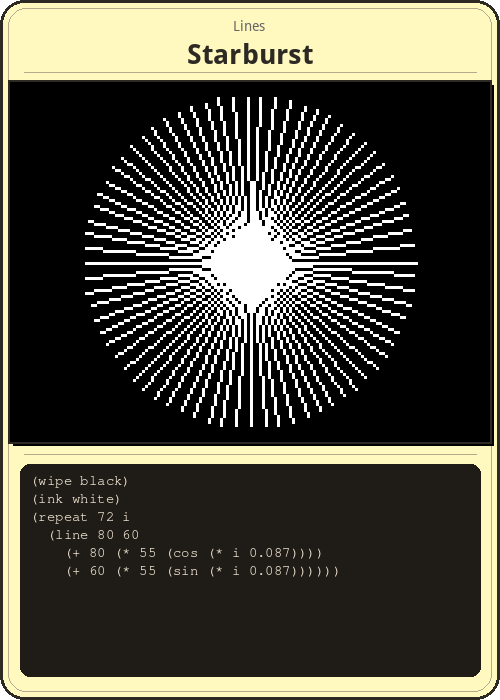
\includegraphics[width=0.47\columnwidth]{card-starburst.png}}%
\hfill%
\fbox{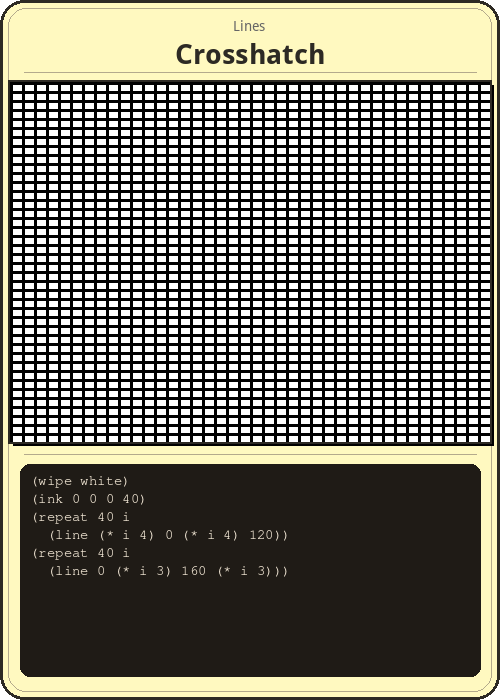
\includegraphics[width=0.47\columnwidth]{card-crosshatch.png}}
\caption{``Starburst'' と ``Crosshatch'' --- 線カード。}
\label{fig:lines}
\end{figure}

\begin{lstlisting}
; Starburst — 72 radial lines
(wipe |\kt{black}|)
(ink |\kt{white}|)
(repeat |\kn{72}| |\kv{i}|
  (line |\kn{80}| |\kn{60}|
    (|\km{+}| |\kn{80}| (|\km{*}| |\kn{55}| (|\km{cos}| (|\km{*}| |\kv{i}| |\kn{0.087}|))))
    (|\km{+}| |\kn{60}| (|\km{*}| |\kn{55}| (|\km{sin}| (|\km{*}| |\kv{i}| |\kn{0.087}|))))))
\end{lstlisting}

\subsection{円}

円カードは \texttt{outline} モードとネストされた \texttt{repeat} ループを使用する。``Ripple'' は30個の同心円を描き、色が青方向にグラデーションする。

\begin{figure}[h]
\centering
\fbox{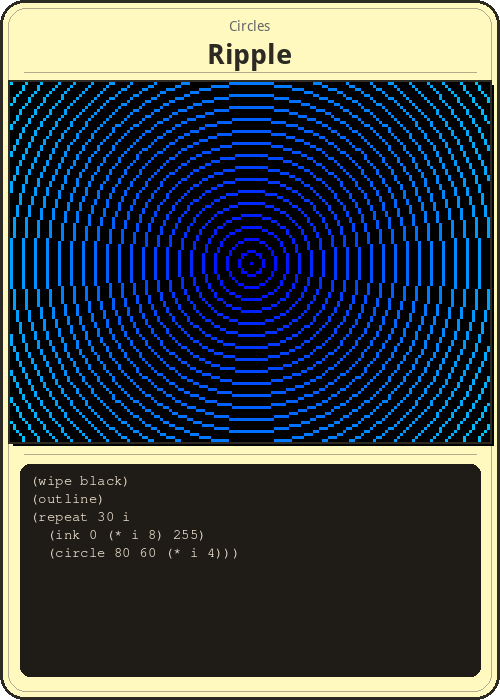
\includegraphics[width=0.47\columnwidth]{card-ripple.png}}%
\hfill%
\fbox{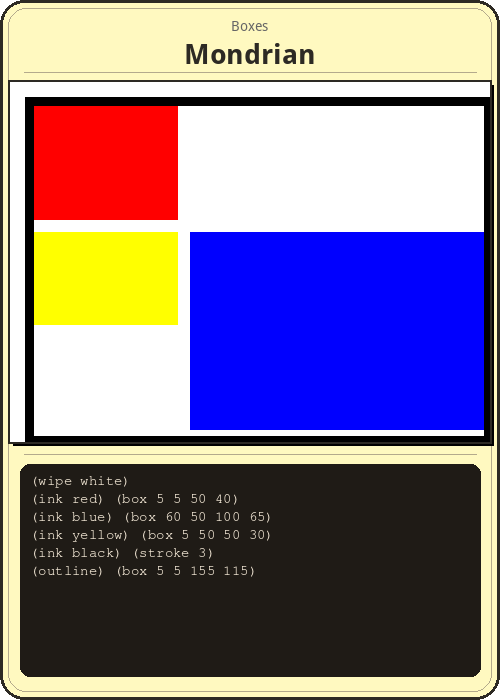
\includegraphics[width=0.47\columnwidth]{card-mondrian.png}}
\caption{``Ripple''（円）と ``Mondrian''（ボックス）。}
\label{fig:circles-boxes}
\end{figure}

\subsection{ボックスと構図}

``Mondrian'' は4つの色付き矩形で原色グリッドを再現する。``Nest'' は10個のネストされた矩形を色相を変化させながら描く。

\subsection{数学と曲線}

これらのカードは \texttt{plot} と数学関数を使用する。``Lissajous'' は600点でリサジュー図形を描く。``Spiral'' は極座標の螺旋線を描く。

\begin{figure}[h]
\centering
\fbox{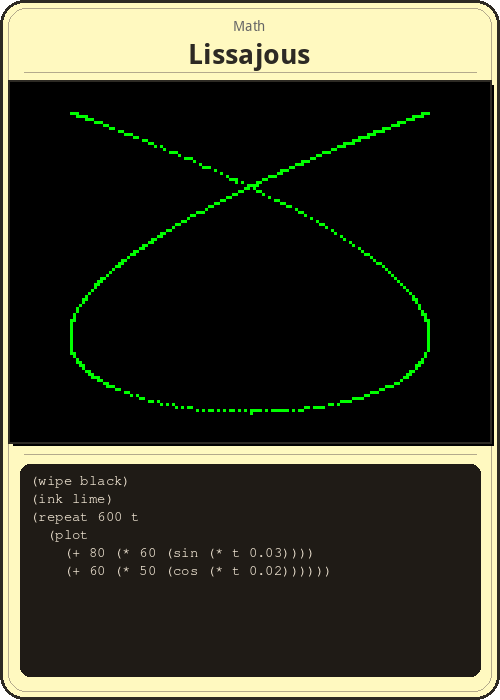
\includegraphics[width=0.47\columnwidth]{card-lissajous.png}}%
\hfill%
\fbox{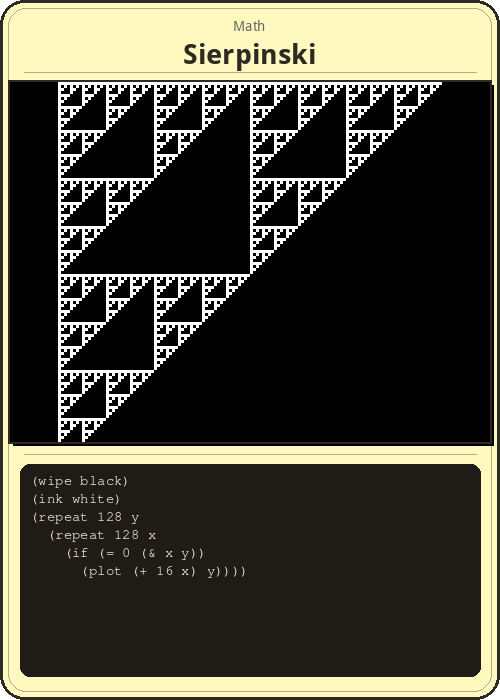
\includegraphics[width=0.47\columnwidth]{card-sierpinski.png}}
\caption{``Lissajous''（数学曲線）と ``Sierpinski''（ビット演算フラクタル）。}
\label{fig:math}
\end{figure}

\subsection{色とグラデーション}

``Sierpinski'' はビット演算AND操作でシェルピンスキー三角形を生成する：\texttt{(if (= 0 (\& x y)) (plot (+ 16 x) y))}。``Sunflower'' は黄金角の螺旋に沿って500点を色の循環とともに描く。

\subsection{タートルグラフィックス}

タートルカードは \texttt{crawl}、\texttt{left}、\texttt{right}、\texttt{face} を使用する。五芒星は \texttt{(right 144)} を使う。木は \texttt{later} で再帰的に分岐する。雪の結晶はコッホ曲線セグメントをネストする。

\begin{figure}[h]
\centering
\fbox{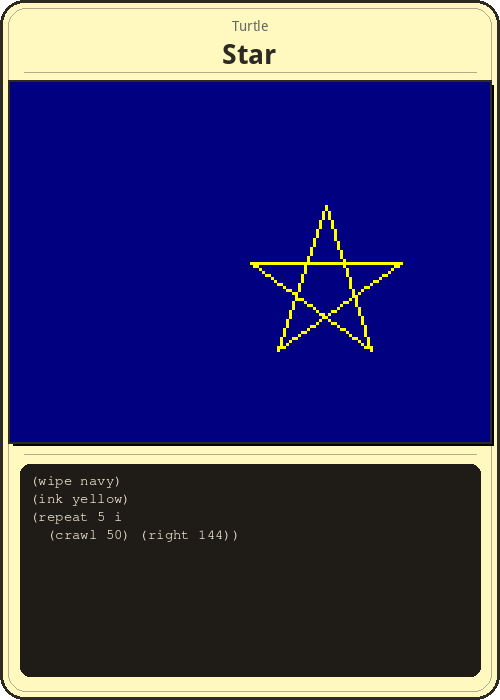
\includegraphics[width=0.47\columnwidth]{card-star.png}}%
\hfill%
\fbox{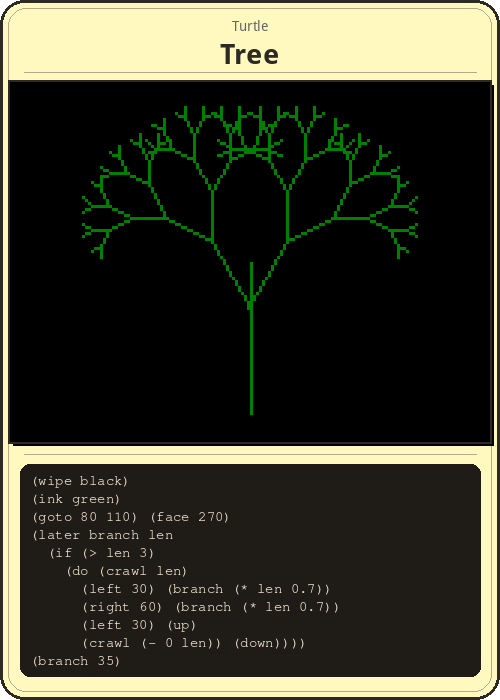
\includegraphics[width=0.47\columnwidth]{card-tree.png}}
\caption{``Star'' と ``Tree'' --- タートルグラフィックスカード。}
\label{fig:turtle}
\end{figure}

\begin{lstlisting}
; Star — 5 sides, 144-degree turns
(wipe |\kt{navy}|)
(ink |\kt{yellow}|)
(repeat |\kn{5}| |\kv{i}| (crawl |\kn{50}|) (right |\kn{144}|))
\end{lstlisting}

\subsection{ミニマル公案}

デッキの中で最も短いカード。``Horizon'' は3行：暗い空、金色の大地。``Pip'' は黒の上に赤い一点。これらのカードは最小限のプログラムに接近する——認識可能な画像を生み出すのに必要な最少コード量。

\begin{figure}[h]
\centering
\fbox{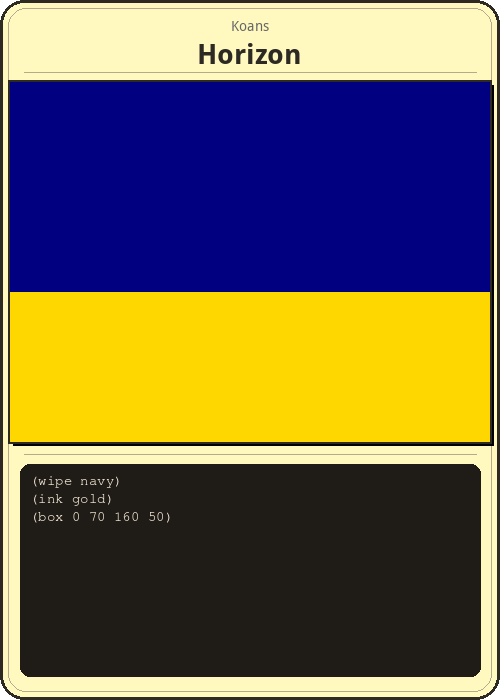
\includegraphics[width=0.47\columnwidth]{card-horizon.png}}%
\hfill%
\fbox{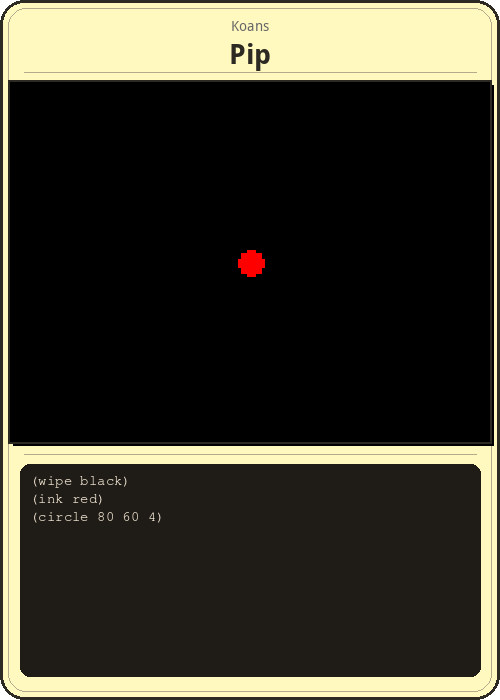
\includegraphics[width=0.47\columnwidth]{card-pip.png}}
\caption{``Horizon'' と ``Pip'' --- ミニマル公案（各2--3行）。}
\label{fig:koans}
\end{figure}

\begin{lstlisting}
; Pip — the minimum card
(wipe |\kt{black}|)
(ink |\kt{red}|)
(circle |\kn{80}| |\kn{60}| |\kn{4}|)
\end{lstlisting}

\begin{figure*}[t]
\centering
\fbox{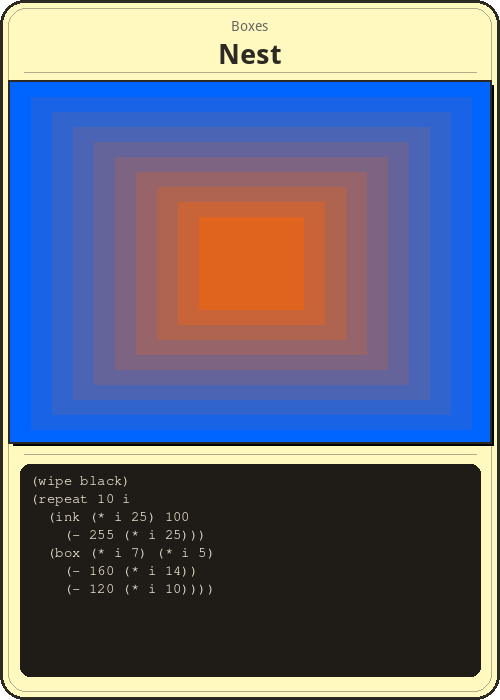
\includegraphics[height=5.5cm]{card-nest.png}}%
\hfill%
\fbox{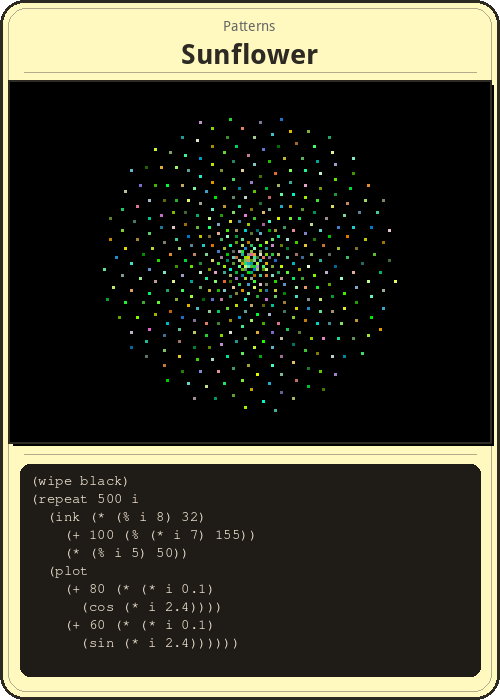
\includegraphics[height=5.5cm]{card-sunflower.png}}%
\hfill%
\fbox{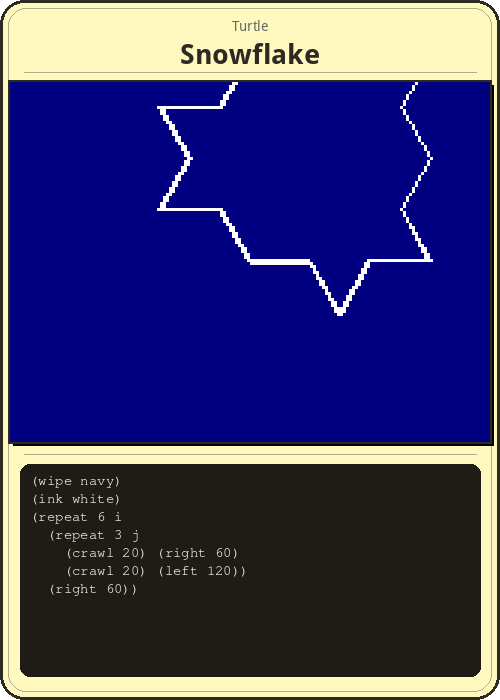
\includegraphics[height=5.5cm]{card-snowflake.png}}%
\hfill%
\fbox{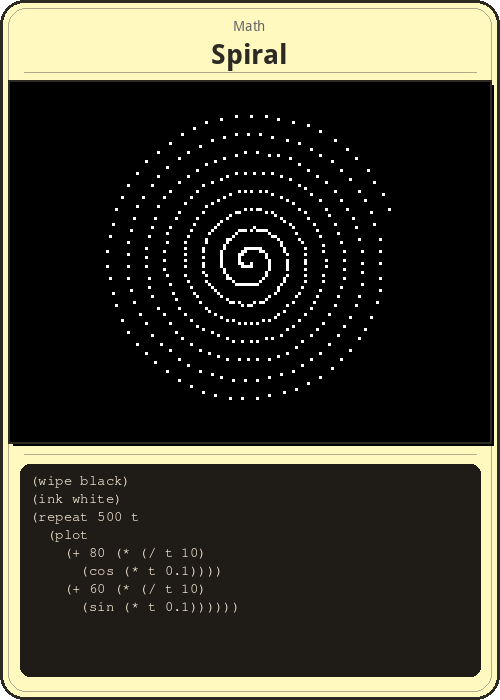
\includegraphics[height=5.5cm]{card-spiral.png}}
\caption{フォーマットを示す4枚の完全なカード：タイトル、レンダリング出力、ソースコード。左から右へ：``Nest''、``Sunflower''、``Snowflake''、``Spiral''。各カードは自己完結している——画像下のソースコードが完全なプログラムである。これらはシンプルな描画演習であり、フォーマットの潜在力の表現ではない。}
\label{fig:four-cards}
\end{figure*}

% ============ 5. レイアウト ============

\section{レイアウト}
\label{sec:layouts}

カードフォーマットに固定レイアウトはない。3つの要素（タイトル、出力、ソースコード）の配置がカードのアフォーダンス——物理的・社会的に何ができるかを決定する。本節ではレイアウトバリエーションとその帰結を探求する。

\begin{figure*}[t]
\centering
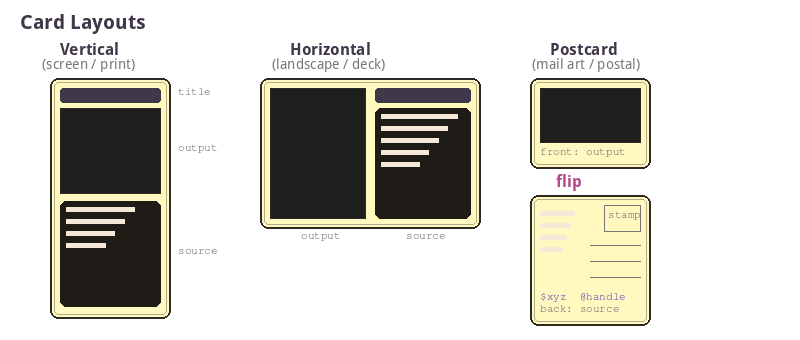
\includegraphics[width=\textwidth]{layout-comparison.png}
\caption{3つのレイアウト戦略。\textbf{縦型：}タイトル/画像/ソースコードを上から下に積み重ね、携帯画面と縦型印刷に最適化。\textbf{横型：}画像を左に、タイトルとソースコードを右に配置し、横型カードと並列閲覧に適する。\textbf{ポストカード：}表面にレンダリング出力、裏面にソースコードとメタデータ——裏返すまでプログラムが見えない郵送可能なカード。}
\label{fig:layouts}
\end{figure*}

\subsection{縦型（画面/印刷）}

デフォルトレイアウトはタイトル、画像、ソースコードを上から下に積み重ねる。これはノートブックレイアウト——携帯電話やJupyterノートブックで自然にスクロールできる。印刷用には4$\times$6インチの縦型カードに対応。読者の目は名前から画像、コードへと下に移動し、プログラムとその出力の関係をたどる。

\subsection{横型（デッキ/風景）}

横型レイアウトはレンダリング画像を左に、ソースコードを右に配置する。テーブルに広げたカード、スライドプレゼンテーション、並列比較に適する。2枚のカードを横に並べるとディプティック——観者がプログラムと出力を同時に比較できる。

\subsection{ポストカード（メールアート）}

ポストカードレイアウトは表と裏を分離する。表面はレンダリング画像のみ、裁ち落とし、テキストなし。裏面にソースコード、作者クレジット、ショートコード（\texttt{\$xyz}）、切手エリア。受取人はまず画像を見る——ビジュアルアーティファクト。カードを裏返すとプログラムが現れる：それを生成した指示。カードは読む面によってアート作品でもあり実行可能なスコアでもある。

\begin{figure*}[h]
\centering
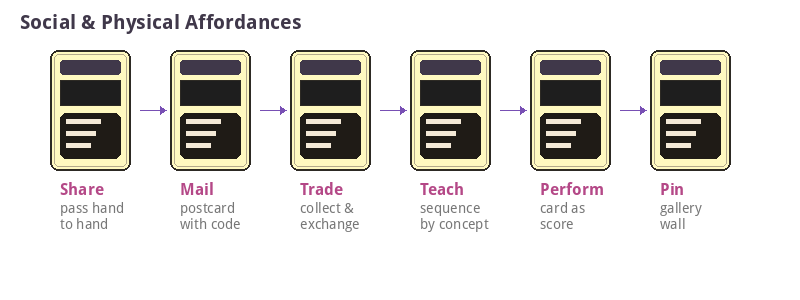
\includegraphics[width=\textwidth]{layout-affordances.png}
\caption{カードフォーマットの社会的・物理的アフォーダンス。各アフォーダンスはカードの物質性に由来する：手渡しで\textbf{共有}、ポストカードとして\textbf{郵送}、\textbf{交換}して収集、教育シーケンスで\textbf{教育に使用}、グラフィックスコアとして\textbf{演奏}、ギャラリーの壁に\textbf{貼る}。}
\label{fig:affordances}
\end{figure*}

\subsection{デッキ編成}

カードは単独のオブジェクトではない。デッキを形成し、デッキの編成が意味を生み出す。\emph{教育シーケンス}はカードを概念順に並べる：まずボックス（座標）、次に線（三角関数）、円（半径と繰り返し）、数学曲線（plotと正弦）、タートルグラフィックス（相対運動）、最後に公案（ミニマルな表現）。\emph{ギャラリーグリッド}はカードを壁面上に空間配置し、カテゴリ間の比較を誘う。\emph{シャッフルデッキ}は順序をランダム化し、フラクタルと地平線の間、木と点の間に予想外の並置を生む。

\begin{figure}[h]
\centering
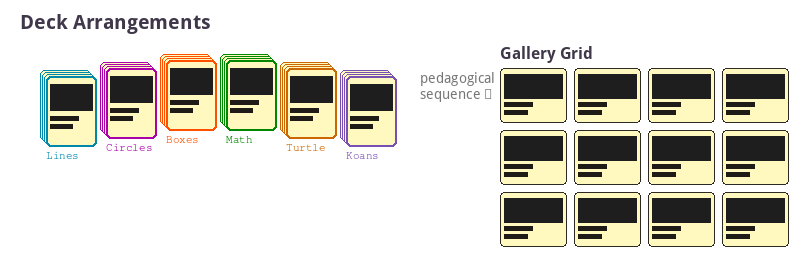
\includegraphics[width=\columnwidth]{layout-decks.png}
\caption{デッキ編成。左：カテゴリ別に展開されたカード（線、円、ボックス、数学、タートル、公案）、各カテゴリに複数のカードが重ねられている。右：閲覧用に空間配置されたギャラリーグリッド。}
\label{fig:decks}
\end{figure}

% ============ 6. 実際のカード ============

\section{実際のカード}
\label{sec:wild}

ノートブックのカードは練習問題である。本当の \kidlisp{} コーパス——59人の作者が作った16,000以上のプログラム——には完全なランタイムを使用する作品が含まれる：アニメーション、オーディオ、埋め込みレイヤー、グラデーションフェード、ランダム配置、タイミング構文。これらの作品はカードフォーマットに収まるほど短いが、ノートブックの例よりはるかに表現力豊かである。プレビュー画像はovenサービス（Puppeteerベースのスクリーンキャプチャ）でレンダリングされ、CDN経由で配信される。

\begin{figure*}[t]
\centering
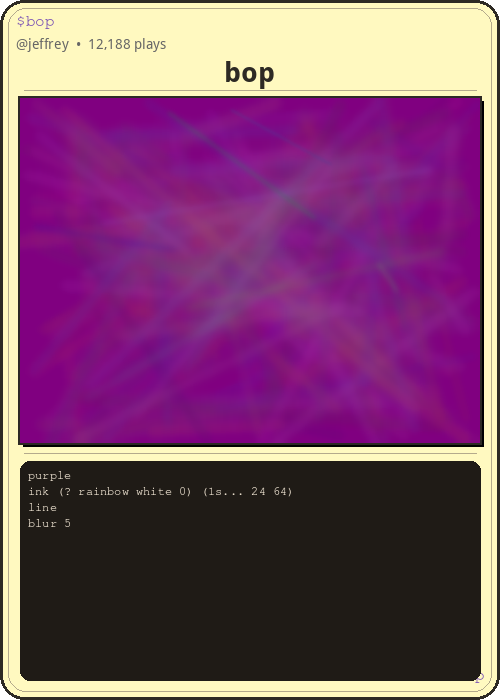
\includegraphics[height=7cm]{user-card-bop.png}%
\hfill%
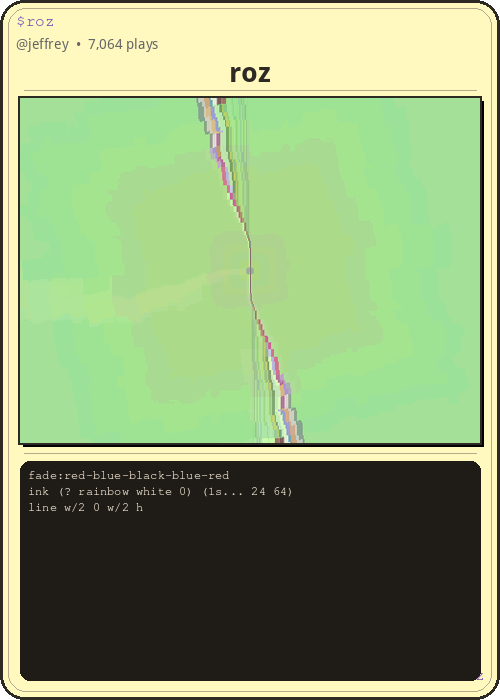
\includegraphics[height=7cm]{user-card-roz.png}%
\hfill%
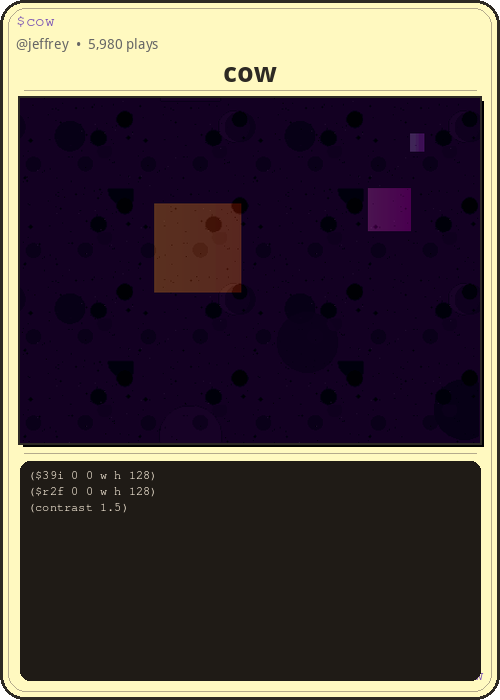
\includegraphics[height=7cm]{user-card-cow.png}%
\hfill%
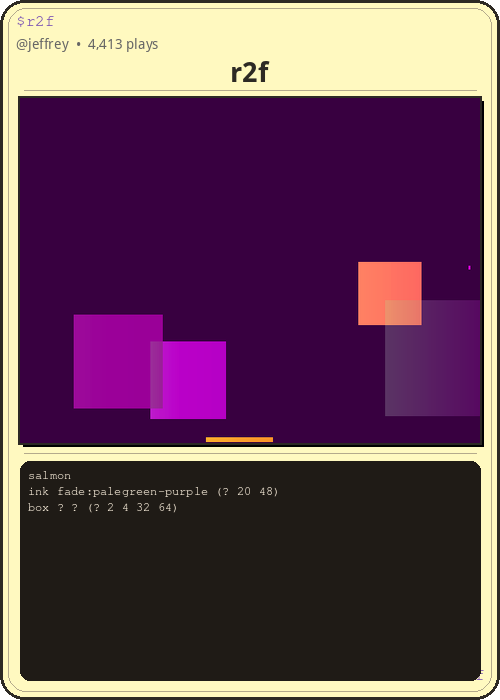
\includegraphics[height=7cm]{user-card-r2f.png}
\caption{\kidlisp{} のアクティブコーパスからの4枚のカード、ovenサービスでレンダリング。左から右へ：\texttt{\$bop}（12,188再生——最も人気のある作品、4行）、\texttt{\$roz}（7,064再生、3行）、\texttt{\$cow}（5,980再生——\texttt{\$39i} と \texttt{\$r2f} を通じて他の2つの作品を埋め込む合成作品）、\texttt{\$r2f}（4,413再生、3行のランダムボックス配置）。すべて@jeffreyの作品。これらのプログラムはPythonインタプリタにはない機能——アニメーション、ランダム性（\texttt{?}）、グラデーションフェード（\texttt{fade:}）、埋め込みレイヤー（\texttt{\$code}）——を使用するが、ソースコードは依然として1枚のカードに収まる。}
\label{fig:user-cards}
\end{figure*}

\subsection{実作品が加えるもの}

ノートブックのカードは \kidlisp{} の静的サブセットを使用する。\texttt{kidlisp.com} 上の実作品は完全なランタイムを使用する：

\begin{itemize}
  \item \textbf{アニメーション。}プログラムは毎フレーム再評価される。\texttt{frame} と \texttt{time} が自動変化。シングルフレームのスクリーンショットはアクティブな作品の一瞬を捉える。
  \item \textbf{ランダム性。}\texttt{?} 演算子は毎フレームリストからランダムな値を生成。\texttt{(ink (? red blue green))} は色間をフリッカーする。
  \item \textbf{グラデーションフェード。}\texttt{fade:red-blue-black} はキャンバス上でマルチストップグラデーションを \texttt{frame} カウント駆動で補間。1つの式が何ページもの手動色計算を置き換える。
  \item \textbf{埋め込み。}\texttt{(\$cow)} はMongoDBから作品 \texttt{cow} を取得し、オフスクリーンバッファで評価し、結果を合成。作品が作品の上に構築される。
  \item \textbf{タイミング。}\texttt{1s... (zoom 0.5)} は毎秒ズームを適用。明示的なアニメーションループ不要。
\end{itemize}

これらの機能はプログラムを短く保ちつつ表現力を劇的に拡張する。\texttt{\$bop}——最も再生された作品、12,188回視聴——はわずか4行：紫の背景、虹色に点滅するインク、ランダムな線、ブラー。カード上では動的な絵画のフリーズフレームに見える。ブラウザではまさにそれである。

\subsection{スナップショットとしてのカード}

アニメーション作品のカードは必然的に不完全である。時間的プロセスの1フレームを捉える。この不完全さはフォーマットの一部である：カードはコードを入力して実際に何をするか見ることを誘う。静止画像は約束。ソースコードは履行。ショートコード（\texttt{\$bop}）は架け橋——\texttt{kidlisp.com} で入力すれば、カードが生き返る。

% ============ 7. カードが将来なりうるもの ============

\section{カードが将来なりうるもの}
\label{sec:futures}

カードフォーマットはまだ若い。現在のノートブックはコンセプト実証——オフラインレンダリングされた28のプログラム。しかし短いプログラムと物理カードの対応はいくつかの方向を示唆する。

\subsection{トレーディングカード}

KidLispカードはほとんどのソフトウェアにはないコレクション性を持つ。各カードに名前、ビジュアルアイデンティティ、ショートコード（\texttt{\$xyz}）、作者がある。カードは印刷、番号付け、交換が可能。レアカードは珍しい言語機能を使ったり、最小限のコードから予想外の複雑な出力を生み出したりするかもしれない。カードの「レア度」はその情報密度：何文字からどれだけのビジュアル複雑性が創発するか。

\subsection{教育シーケンス}

現在のノートブックの7つのカテゴリは教育的順序を示唆する：ボックスから始め（単純な座標）、線（三角関数）、円（半径と繰り返し）、数学曲線（plotと正弦）、タートルグラフィックス（相対運動）、最後に公案（ミニマルな表現）へ進む。各カードが1つの概念を教える。教師は実物のカードデッキを生徒に渡し、各カードを再現したり、修正したり、同じカテゴリで新しいカードを作ったりするよう求めることができる。

\subsection{印刷スコア}

音楽において、スコアは時間的イベントを生成する指示である。KidLispカードはビジュアルイベントを生成する指示である。カードはグラフィックスコアとして機能しうる——Cornelius Cardew、John Cage、Fluxusイベントスコアの伝統に連なる。演奏者はカードを受け取り、コードを解釈（\texttt{kidlisp.com} で入力、声に出して読む、手で描く）し、イベントを生み出す。カードがスコアであり、レンダリングはその一つの可能な実現である。

\subsection{メールアート}

4$\times$6インチのKidLispカードはポストカードそのものである。表面にレンダリング画像。裏面にソースコード、作者クレジット、オンラインで見つけるためのショートコード。実行可能な内容を持つメールアート——受取人はコードを入力して自分のスクリーンで画像が再生成されるのを見ることができる。物理カードとデジタルプログラムは同じ作品の2つの媒体である。

\subsection{ジェネラティブ文房具}

Pythonインタプリタは確定的で独立して動作するため、ネットワークアクセスなしで印刷制作用にカードをバッチレンダリングできる。カードセットは小冊子、独立出版物、ボックスセットとして印刷可能。\texttt{cards-convert.mjs} パイプラインはすでに論文フォーマットから4$\times$6インチPDFカードを生成できる。レンダリングされたプログラム出力とソースコードの両方を含むよう拡張するのは自然な次のステップである。

\subsection{生成原理としての制約}

カードフォーマットの最も興味深い帰結は、言語へのフィードバック方法である。カードに収まらないプログラムは欠けている抽象化を示唆する——あるいはプログラムがやりすぎていることを示唆する。カード制約は経済性を促す：最も興味深い画像を生む3行のプログラムを見つけよ。これはOulipo的な生成的制約——任意の形式的制限が予想外の創造的結果を生む。

% ============ 6. 関連研究 ============

\section{関連研究}

\textbf{印刷されたコード。}デモシーンの「sizecoding」の伝統（256バイト以下のプログラム）は、最小のプログラムから最大の出力を得る美学と共鳴する。\kidlisp{} カードは「コードポエトリー」の伝統により近い——ソースコード自体がその出力とともにテキストとして読まれる。

\textbf{グラフィックスコア。}Cardewの\emph{Treatise}（1967）とCageの\emph{Notations}（1969）は、ビジュアル記法が特定の実現を規定せずに演奏指示として機能しうることを確立した。KidLispカードの違いは完全に実行可能であること——レンダリングは確定的で解釈に開かれていない。しかしカード即スコアのフレームワークは再解釈を誘う：もし毎回異なる方法でカードを「演奏」したら？

\textbf{トレーディングカードゲーム。}\emph{Magic: The Gathering}（1993）などのゲームは、構造化されたメタデータ（名前、タイプ、ルールテキスト、イラスト）を持つカードが豊かな組み合わせ空間を生み出すことを実証した。KidLispカードは自然なメタデータ（タイトル、カテゴリ、関数数、行数、出力の複雑さ）を持ち、類似のゲームメカニクスをサポートできる。

\textbf{計算ノートブック。}Jupyterノートブックはすでにコードと出力を組み合わせている。KidLisp Cardsノートブックは特定の制約を持つJupyterノートブックである：各セルはより長い計算のステップではなく自己完結したカード。ノートブックはナラティブではなくギャラリーである。

% ============ 7. 結論 ============

\section{結論}

KidLispカードはシンプルな観察に由来する：プログラムが十分に短ければ、カードに収まる。カードフォーマット——タイトル、画像、ソースコード——はプログラムを印刷、郵送、収集、教育、演奏できる物理的アーティファクトに変える。Pythonレンダリングパイプラインがオフラインバッチ制作を可能にする。7カテゴリのカタログが言語へのキュレーションされた入り口を提供する。

フォーマットは進行中の作品である。現在の28枚のデッキは出発点であり、完成したコレクションではない。問題は何枚カードを作るかではなく、どのプログラムがカードになる価値があるか——手に取る価値のある画像を生み出す3行の構図はどれか。

ノートブック、インタプリタ、カードカタログは \url{https://github.com/whistlegraph/aesthetic-computer} で入手可能。プログラムは \url{https://kidlisp.com} で作成・共有できる。

\vspace{0.5em}
\noindent\textbf{ORCID:} \href{https://orcid.org/0009-0007-4460-4913}{0009-0007-4460-4913}

% ============ 参考文献 ============

\bibliographystyle{plainnat}
\bibliography{references}

\end{document}
